\documentclass{article}
\usepackage{graphicx}
\usepackage{booktabs}
\usepackage{tabularx}
\usepackage{hyperref}
\usepackage{pdflscape}

\hypersetup{
    colorlinks=true,       % false: boxed links; true: colored links
    linkcolor=red,          % color of internal links (change box color with linkbordercolor)
    citecolor=green,        % color of links to bibliography
    filecolor=magenta,      % color of file links
    urlcolor=cyan           % color of external links
}

\title{Hazard Analysis\\\progname}

\author{\authname}

\date{}

%% Comments

\usepackage{color}

\newif\ifcomments\commentstrue %displays comments
%\newif\ifcomments\commentsfalse %so that comments do not display

\ifcomments
\newcommand{\authornote}[3]{\textcolor{#1}{[#3 ---#2]}}
\newcommand{\todo}[1]{\textcolor{red}{[TODO: #1]}}
\else
\newcommand{\authornote}[3]{}
\newcommand{\todo}[1]{}
\fi

\newcommand{\wss}[1]{\authornote{blue}{SS}{#1}} 
\newcommand{\plt}[1]{\authornote{magenta}{TPLT}{#1}} %For explanation of the template
\newcommand{\an}[1]{\authornote{cyan}{Author}{#1}}

%% Common Parts

\newcommand{\progname}{Software Engineering} % PUT YOUR PROGRAM NAME HERE
\newcommand{\authname}{Team 2, SyntaxSentinals
\\ Lucas Chen
\\ Dennis Fong
\\ Mohammad Mohsin Khan
\\ Julian Cecchini
\\ Luigi Quattrociocchi} % AUTHOR NAMES                  

\usepackage{hyperref}
    \hypersetup{colorlinks=true, linkcolor=blue, citecolor=blue, filecolor=blue,
                urlcolor=blue, unicode=false}
    \urlstyle{same}
                                


\begin{document}

\maketitle
\thispagestyle{empty}

~\newpage

\pagenumbering{roman}

\begin{table}[hp]
\caption{Revision History} \label{TblRevisionHistory}
\begin{tabularx}{\textwidth}{llX}
\toprule
\textbf{Date} & \textbf{Developer(s)} & \textbf{Change}\\
\midrule
Oct 15 & SyntaxSentinels & Initial Revision\\
... & ... & ...\\
\bottomrule
\end{tabularx}
\end{table}

~\newpage

\tableofcontents

~\newpage

\pagenumbering{arabic}

\wss{You are free to modify this template.}

\section{Introduction}

% \wss{You can include your definition of what a hazard is here.}
A hazard is a property or condition in the system together with a condition in the environment that has the potential to cause harm, disrupt operations, 
or negatively affect the functionality of a system. Hazards can arise from various sources, including system 
malfunctions, human errors, environmental factors, or security vulnerabilities.

This document is the hazard analysis for the Capstone SyntaxSentinels. This project seeks to create a plagiarism algorithm that relies on NLP
techniques of present to account for semantics and prevent primitive circumvention of plagiarism detection, such as the addition of benign lines or
variable name changes.

\section{Scope and Purpose of Hazard Analysis}

\wss{You should say what \textbf{loss} could be incurred because of the
hazards.}

\section{System Boundaries and Components}

\hspace*{-3cm}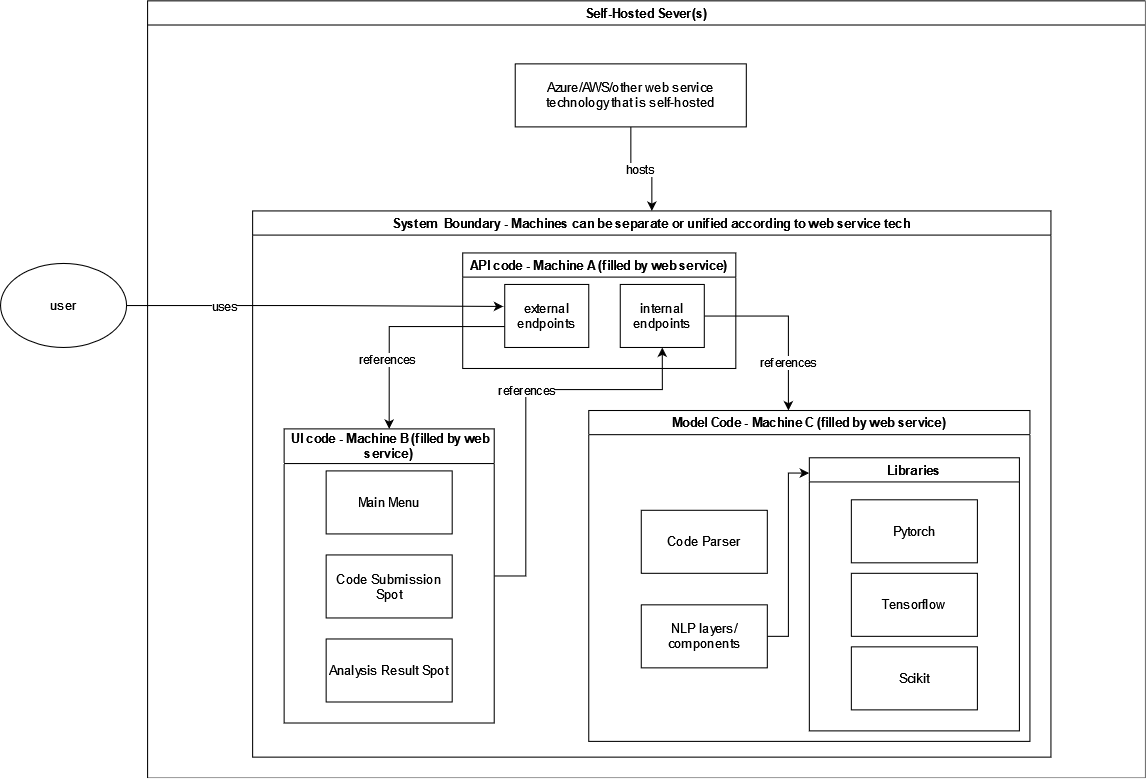
\includegraphics[height=.58\textheight]{./assets/Component_Border.png}

Diagram shows referential relationships, not workflows. System Boundary above surrounds all components our team will maintain and accept responsibility. A machine above is a server suitable to host code specified. Any machine mentioned above will not be provided to users from our project, they are expected to be self-hosted either on the user's own servers, or through technology such as Amazon Web Services (AWS) or Microsoft Azure.

\section{Critical Assumptions}
\begin{itemize}
    \item Adequate computational resources exist for the real time analysis of the code snippets
    \item Users do not intend to misuse the product
    \item Third party resources that support this product will always be functionally correct
    \item All components on the cloud will provide sufficient scalability and security
    \item The system will be maintained regularly with bug fixes/performance enhancements
    \item The criteria for plagiarism is agreed upon by all users
\end{itemize}

\section{Failure Mode and Effect Analysis}

\begin{landscape}
    \begin{table}[ht]
        \centering
        \scalebox{0.7}{ 
        \begin{tabular}{|p{1.75cm}|p{4cm}|p{5cm}|p{5cm}|p{3cm}|p{5cm}|p{2cm}|p{2cm}|}
        \hline
        \textbf{Design Function} & \textbf{Failure Modes} & \textbf{Effects of Failure} & \textbf{Causes of Failure} & \textbf{Detection} & \textbf{Recommended Actions} & \textbf{SR} & \textbf{Ref.} \\
        \hline
        Input Processing & Failure to tokenize text & Model fails to function or gives wrong output & a. Code not in Python \newline b. Tokenizer malfunction \newline c. Corrupted file & Check file extension to ensure .py suffix & a. Check input beforehand \newline b. Notify user of error occurred & & \\
        \cline{2-8}
        & Failure to upload file & Plagiarism detection process does not start & a. Invalid file type \newline b. Server error & Error handling & a. Notify user of failed upload & & \\
        \cline{2-8}
        \hline
        User Account Handling & Unauthorized access to account & a. Account compromised \newline b. User submissions compromised & a. Weak user authentication measures &  & a. Limit unsuccessful login attempts \newline  b. Multi-factor authentication & & \\
        \cline{2-8}
        \hline
        Result processing and generation & Model is overfitted & Model fails to identify plagiarism for many inputs & a. Small dataset \newline b. Dataset too specific  & Test model with test dataset & a. Ensure datasets don't all have similar code & & \\
        \cline{2-8}
        & Model providing false positives & Submissions incorrectly flagged for plagiarism & a. Inability to recognize common coding practices \newline b. Error in model & Proper tests with test data split & a. Implement good pattern analysis \newline b. Proper testing & & \\
        \cline{2-8}
        & Comments are tokenized or ignored incorrectly & Comments become extremely easy way to bypass plagiarism detection & a. Bad implementation of model \newline b. Error in code & Found in testing using inputs with comments & a. Ensure code handles comments properly & &\\
        \hline
        Result output display & Results e-mail failed to send & Users who close the tab will not see the results & a. Network issues on either sender/recipient side \ newline b. Blocked by spam filters \newline c. Incorrect e-mail address & & a. Send e-mail from safe and trusted domains b. Ensure recipient address is filled correctly in script & & \\
        \hline
        \end{tabular}
        } % End of \scalebox
        \caption{Failure Mode and Effect Analysis}
        \label{table:fmea}
    \end{table}
\end{landscape}
   

\section{Safety and Security Requirements}

\wss{Newly discovered requirements.  These should also be added to the SRS.  (A
rationale design process how and why to fake it.)}

\section{Roadmap}

\wss{Which safety requirements will be implemented as part of the capstone timeline?
Which requirements will be implemented in the future?}

\newpage{}

\section*{Appendix --- Reflection}

\wss{Not required for CAS 741}

The purpose of reflection questions is to give you a chance to assess your own
learning and that of your group as a whole, and to find ways to improve in the
future. Reflection is an important part of the learning process.  Reflection is
also an essential component of a successful software development process.  

Reflections are most interesting and useful when they're honest, even if the
stories they tell are imperfect. You will be marked based on your depth of
thought and analysis, and not based on the content of the reflections
themselves. Thus, for full marks we encourage you to answer openly and honestly
and to avoid simply writing ``what you think the evaluator wants to hear.''

Please answer the following questions.  Some questions can be answered on the
team level, but where appropriate, each team member should write their own
response:


\begin{enumerate}
    \item What went well while writing this deliverable? 
    \item What pain points did you experience during this deliverable, and how
    did you resolve them?
    \item Which of your listed risks had your team thought of before this
    deliverable, and which did you think of while doing this deliverable? For
    the latter ones (ones you thought of while doing the Hazard Analysis), how
    did they come about?
    \item Other than the risk of physical harm (some projects may not have any
    appreciable risks of this form), list at least 2 other types of risk in
    software products. Why are they important to consider?
\end{enumerate}

\end{document}